\documentclass[conf]{new-aiaa}
%\documentclass[journal]{new-aiaa} for journal papers
\usepackage[utf8]{inputenc}

\usepackage{graphicx}
\usepackage{amsmath}
\usepackage[version=4]{mhchem}
\usepackage{siunitx}
\usepackage{longtable,tabularx}
\setlength\LTleft{0pt} 

\title{Preparation of Papers for AIAA Technical Conferences}

\author{First A. Author\footnote{Insert Job Title, Department Name, Address/Mail Stop, and AIAA Member Grade (if any) for first author.} and Second B. Author Jr.\footnote{Insert Job Title, Department Name, Address/Mail Stop, and AIAA Member Grade (if any) for second author.}}
\affil{Business or Academic Affiliation 1, City, State, Zip Code}
\author{Third C. Author\footnote{Insert Job Title, Department Name, Address/Mail Stop, and AIAA Member Grade (if any) for third author.}}
\affil{Business or Academic Affiliation 2, City, Province, Zip Code, Country}
\author{Fourth D. Author\footnote{Insert Job Title, Department Name, Address/Mail Stop, and AIAA Member Grade (if any) for fourth author (etc.).}}
\affil{Business or Academic Affiliation 2, City, State, Zip Code}

\begin{document}

\maketitle

\begin{abstract}
These instructions give you guidelines for preparing papers for AIAA Technical Papers using \LaTeX{}. Define all symbols used in the abstract. Do not cite references in the abstract. The footnote on the first page should list the Job Title and AIAA Member Grade for each author, if known Authors do not have to be AIAA members.
\end{abstract}

\section{Nomenclature}

{\renewcommand\arraystretch{1.0}
\noindent\begin{longtable*}{@{}l @{\quad=\quad} l@{}}
$A$  & amplitude of oscillation \\
$a$ &    cylinder diameter \\
$C_p$& pressure coefficient \\
$Cx$ & force coefficient in the \textit{x} direction \\
$Cy$ & force coefficient in the \textit{y} direction \\
c   & chord \\
d$t$ & time step \\
$Fx$ & $X$ component of the resultant pressure force acting on the vehicle \\
$Fy$ & $Y$ component of the resultant pressure force acting on the vehicle \\
$f, g$   & generic functions \\
$h$  & height \\
$i$  & time index during navigation \\
$j$  & waypoint index \\
$K$  & trailing-edge (TE) nondimensional angular deflection rate
\end{longtable*}}

\section{Introduction}
\lettrine{T}{his} document is a \LaTeX{} template for preparation of papers for AIAA Technical Conferences. If you are reading a hard-copy or .pdf version of this document, download the electronic file, new-aiaa.cls, and use it to prepare your manuscript.

Authors using \url{https://www.overleaf.com} may simply open the AIAA template from the Overleaf gallery to work online; no local installation of any files is required. Authors using a local \LaTeX{} installation will need to open the template in Overleaf and use the ``Download as zip'' option from the project menu to download a local copy of the template files. To create your formatted manuscript, type your own text over sections of the template, or cut and paste from another document and then use the available markup styles. Note that special formatting such as subscripts, superscripts, and italics may be lost when you copy your text into the template from a Word Processing program such as Microsoft Word. See Sec. V for more detailed formatting guidelines.

\section{Procedure for Paper Submission}

All manuscripts are to be submitted electronically to the ScholarOne Abstracts site created for each conference. The manuscript upload will be enabled several weeks after acceptance notices have been sent. Presenting authors of accepted papers will receive an email with instructions when manuscript submission is open. It is important that presenting authors keep their email addresses up-to- date so they do not miss this notice.

Before completing manuscript submission, submitters must also select the copyright statement that will appear on the paper, and complete other acknowledgments. It is also necessary to click both the ``Accept'' and ``Save'' buttons to complete a submission. All completed manuscript submission will be confirmed by email. Completed submissions will also have a status of ``Accepted'' at the top of your manuscript submission page.

All files must be in pdf format. Please be sure that all security settings are removed from the pdf file before uploading to ensure proper processing of your manuscript file.

\section{General Guidelines}

The following section outlines general (nonformatting) guidelines to follow, drawn from the original AIAA Manuscript Preparation Kit. These guidelines are applicable to all authors (except as noted), and include information on the policies and practices relevant to the publication of your manuscript.

\subsection{Publication by AIAA}
Your manuscript cannot be published by AIAA if:
\begin{enumerate}
\item It has been published previously or

\item The work contains copyright-infringing material or

\item An appropriate copyright statement has not yet been selected.
\end{enumerate}

\subsection{Paper Review and Visa Considerations}

It is the responsibility of the author to obtain any required government or company reviews for their papers in advance of publication. Start early to determine if the reviews are required; this process can take several weeks.

If you plan to attend an AIAA Forum, technical conference or professional development course held in the United States and you require a visa for travel, it is incumbent upon you to apply for a visa with the U.S.~embassy (consular division) or consulate with ample time for processing.  To avoid bureaucratic problems, AIAA strongly suggests that you submit your formal application to U.S.~ authorities a minimum of 120 days in advance of the date of anticipated travel.

Prospective conference and course attendees requiring a visa to travel to the United States should first contact

AIAA to request an official letter of invitation. This letter and a copy of the conference call for papers should be presented along with the required documentation to the U.S. consular officials as part of the formal application process.  AIAA cannot directly intervene with the U.S. Department of State, consular offices, or embassies on behalf of individuals applying for visas. A letter of invitation can be requested by completing the Visa Invitation Letter Request Form at \url{https://www.aiaa.org/Secondary.aspx?id=6258} or you may contact the Event Registrar at \url{invitation@aiaa.org} for more information.

\subsection{Control ID Number vs Paper Number}

Your paper was assigned a control ID number at the time you submitted your abstract. It is critical that you reference the tracking number and conference name when contacting AIAA regarding your submission. The control ID number is \emph{not} the final AIAA paper number. The paper number, which appears in the format AIAA-20XX-XXXX, will be used to refer to your paper in the program and in any publication format. It will not be assigned until shortly before the conference. \textbf{Do not include a paper number anywhere on your paper, as this number will be stamped automatically in the top right corner of your paper at the time of processing.}

\subsection{Copyright}

Before AIAA can print or publish any paper, the copyright information must be completed in the submission system. Failure to complete the electronic form correctly could result in your paper not being published. The following fields must be completed:

\begin{enumerate}
\item Clearance Statement
\item Non-Infringement Statement
\item Publication Status Statement
\item One Copyright Assignment Statement (Select either A, B, C, or D)
\end{enumerate}

Be sure to read the copyright statements carefully. AIAA requires a copyright transfer from the author(s) to AIAA or a license to publish and distribute your material; government authors can assert that the work is in the public domain. If you are not sure which copyright statement to use, contact your legal department. Refer to AIAA’s Rights and Permissions page at \url{www.aiaa.org} for more information; AIAA cannot help you determine which statement to use. Do not include a copyright statement anywhere on your paper. A hard copy of the form is found in the Author Kit for your reference. As you will be completing this form online, you do not need to fill out the hard-copy form. Do not include a copyright statement anywhere on your paper, and do not upload a copyright form with your paper. The correct statement will be stamped automatically at the time of processing.

\subsection{Submission Deadlines}

Manuscripts will be accepted for upload to the system from the receipt of the email invitation until the deadline set for the conference. You will be notified of the specific manuscript submission deadline in your acceptance letter, and the deadline will also be listed on the conference web page at AIAA. Please do not upload a draft version of your manuscript with the intent to upload a final version later. \textbf{Please review your manuscript very carefully before completing your submission to ensure that your paper is complete and final in all respects. Once the manuscript deadline has passed you will be locked out of the manuscript site so it is critical that you upload a final, carefully proofed document.}

Online conference proceedings will be made accessible to attendees who have registered for the ``full conference'' when the conference opens. Once the proceedings are published online, the conference papers will be considered the version of record and may not be removed or replaced. Changes to published papers can be made available through the Crossmark feature, where corrections and updates are accessed by clicking the Crossmark icon available on every paper published in Aerospace Research Central.

The opportunity to submit Crossmark updates will be provided to presenting authors starting the first day of the conference through 2000 hrs/8 pm Eastern Time, seven business days after the last day of the conference.  The proceedings will be updated with Crossmark updates shortly after that date.  

AIAA will NOT accept changes and/or change requests that solely correct grammatical errors, spelling errors, or errors in formatting.  All corrections should be for editorially significant changes where the change affects interpretation or crediting of the work.

To ensure conference quality, session chairs will enforce a ``no paper, no podium'' rule. This policy is intended to eliminate no-shows, to improve the quality of the conference for all participants, and to ensure that the published proceedings accurately represent the presentations made at a conference.

\section{Detailed Formatting Instructions}

The styles and formats for the AIAA Papers Template have been incorporated into the structure of this document. If you are using \LaTeX{}, please use this template to prepare your manuscript. A Microsoft Word template is also available from AIAA's website if you prefer to use Microsoft Word 2001 or later. Regardless of which program you use to prepare your manuscript, please use the formatting instructions contained in this document as a guide.

If you are using the AIAA Meeting Papers \LaTeX{} Template file to prepare your manuscript, you can simply type your own text over sections of this document, or cut and paste from another document and use the available markup styles. If you choose to cut and paste, select the text from your original document and choose Edit>Copy. (Do not select your title and author information, since the document spacing may be affected. It is a simple task to reenter your title and author information in the template.) Open the \LaTeX{} template file. Place your cursor in the text area of the template and select Edit>Paste. Please note that special formatting (e.g., subscripts, superscripts, italics) may be lost when you copy your text into the template. Use italics for emphasis; do not underline. Use the compiled \LaTeX{} pdf to see the most accurate representation of how your final paper will appear.

\subsection{Document Text}
The default font for AIAA papers is Times New Roman, 10-point size.  The first line of every paragraph should be indented, and all lines should be single-spaced. Default margins are 1'' on all sides. In the electronic version of this template, all margins and other formatting is preset. There should be no additional lines between paragraphs.

\begin{quoting}
Extended quotes, such as this example, are to be used when material being cited is longer than a few sentences, or the standard quotation format is not practical. In this \LaTeX template, the appropriate command environment is \verb|\begin{quoting}...\end{quoting}|. Extended quotes are to be in Times New Roman, 9-point font, indented 0.4'' and full justified.
\end{quoting}

\emph{NOTE:} If you are using the electronic \LaTeX{} template to format your manuscript, the required spacing and formatting will be applied automatically.

\subsection{Headings}
The title of your paper should be typed in bold, 24-point type, with capital and lower-case letters, and centered at the top of the page. The names of the authors, business or academic affiliation, city, and state/province should follow on separate lines below the title. The names of authors with the same affiliation can be listed on the same line above their collective affiliation information. Author names are centered, and affiliations are centered and in italic type immediately below the author names. The affiliation line for each author is to include that author’s city, state, and zip/postal code (or city, province, zip/postal code and country, as appropriate). The first-page footnotes (lower left-hand side) contain the job title and department name, street address/mail stop, and AIAA member grade for each author. Author email addresses may be included also.

Major headings (``sections'' in the \LaTeX{} template commands) are bold 11-point font, centered, and numbered with Roman numerals.

Subheadings (``subsections'' in the \LaTeX{} template commands) are bold, flush left, and numbered with capital letters. 

Sub-Subheadings (``subsubsections'' in the \LaTeX{} template commands) are italic, flush left, and numbered (1. 2. 3. etc.)


\subsection{Abstract}
The abstract should appear at the beginning of your paper. It should be one paragraph long (not an introduction) and complete in itself (no reference numbers). It should indicate subjects dealt with in the paper and state the objectives of the investigation. Newly observed facts and conclusions of the experiment or argument discussed in the paper must be stated in summary form; readers should not have to read the paper to understand the abstract. The abstract should be bold, indented 3 picas (1/2'') on each side, and separated from the rest of the document by blank lines above and below the abstract text..

\subsection{Nomenclature}
Papers with many symbols may benefit from a nomenclature list that defines all symbols with units, inserted between the abstract and the introduction. If one is used, it must contain all the symbology used in the manuscript, and the definitions should not be repeated in the text. In all cases, identify the symbols used if they are not widely recognized in the profession. Define acronyms in the text, not in the nomenclature.

\subsection{Footnotes and References}
Footnotes, where they appear, should be placed above the 1'' margin at the bottom of the page. To insert footnotes into the template, use the Insert>Footnote feature from the main menu as necessary. Numbered footnotes as formatted automatically in the template are acceptable, but superscript  symbols are the preferred AIAA style, *, $\dag$, $\ddag$, \S, \P, **, $\dag\dag$, $\ddag\ddag$, \S\S, etc.

List and number all references at the end of the paper. Corresponding bracketed numbers are used to cite references in the text \cite{vatistas1986reverse}, including citations that are an integral part of the sentence (e.g., ``It is shown in \cite{dornheim1996planetary} that\ldots '') or follow a mathematical expression: ``$A^{2} + B = C$ (Ref.~\cite{terster1997nasa}).'' For multiple citations, separate reference numbers with commas \cite{peyret2012computational,oates1997aerothermodynamics}, or use a dash to show a range \cite{volpe1994techniques,thompsonspacecraft,chi1993fluid,brandis2016nonequi}. Reference citations in the text should be in numerical order.

In the reference list, give all authors' names; do not use ``et al.''. Papers that have not been published should be cited as ``unpublished''; papers that have been submitted or accepted for publication should be cited as ``submitted for publication.'' Private communications and personal website should appear as footnotes rather than in the reference list.

References should be cited according to the standard publication reference style (for examples, see the ``References'' section of this template). Never edit titles in references to conform to AIAA style of spellings, abbreviations, etc. Names and locations of publishers should be listed; month and year should be included for reports and papers. For papers published in translation journals, please give the English citation first, followed by the original foreign language citation.

\subsection{Images, Figures and Tables}
All artwork, captions, figures, graphs, and tables will be reproduced exactly as submitted. Be sure to position any figures, tables, graphs, or pictures as you want them printed. AIAA will not be responsible for incorporating your figures, tables, etc. (Company logos and identification numbers are not permitted on your illustrations.)

Do not insert your tables and figures in text boxes. Figures should have no background, borders, or outlines. In the \LaTeX{} template, use the ``caption'' command to type caption text. Captions are bold with a single tab (no hyphen or other character) between the figure number and figure description.

% \begin{table}
% \caption{\label{tab:table1} Transitions selected for thermometry}
% \centering
% \begin{tabular}{lcccccc}
% \hline
% & Transition& & \multicolumn{2}{c}{}\\\cline{2-2}
% Line& $\nu''$& & $J'' $& Frequency, cm$^{-1}$& $FJ$, cm$^{-1}$& $G\nu $, cm$^{-1}$\\\hline
% a& 0& P$_{12}$& 2.5& 44069.416& 73.58& 948.66\\
% b& 1& R$_{2}$& 2.5& 42229.348& 73.41& 2824.76\\
% c& 2& R$_{21}$& 805& 40562.179& 71.37& 4672.68\\
% d& 0& R$_{2}$& 23.5& 42516.527& 1045.85& 948.76\\
% \hline
% \end{tabular}
% \end{table}


\begin{figure}[hbt!]
\centering
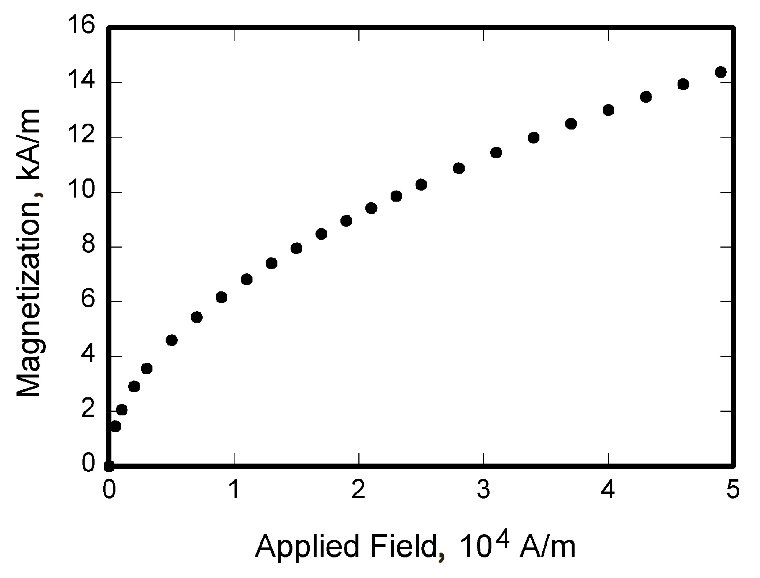
\includegraphics[width=.5\textwidth]{graph}
\caption{Magnetization as a function of applied fields.}
\end{figure}

Place figure captions below all figures; place table titles above the tables. If your figure has multiple parts, include the labels ``a),'' ``b),'' etc. below and to the left of each part, above the figure caption. Please verify that the figures and tables you mention in the text actually exist. \emph{Please do not include captions as part of the figures, and do not put captions in separate text boxes linked to the figures.} When citing a figure in the text, use the abbreviation ``Fig.'' except at the beginning of a sentence. Do not abbreviate ``Table.'' Number each different type of illustration (i.e., figures, tables, images) sequentially with relation to other illustrations of the same type.

Figure axis labels are often a source of confusion. Use words rather than symbols. As in the example to the right, write the quantity ``Magnetization'' rather than just ``M.'' Do not enclose units in parenthesis, but rather separate them from the preceding text by commas. Do not label axes only with units. As in Fig.~1, for example, write ``Magnetization, \si[per-mode=symbol]{\ampere\per\meter},'' not just ``A/m.'' Do not label axes with a ratio of quantities and units. For example, write ``Temperature, K,'' not ``Temperature/K.''

Multipliers can be especially confusing. Write ``Magnetization, \si[per-mode=symbol]{\kilo\ampere\per\meter}'' or ``Magnetization, \SI[per-mode=symbol]{e3}{\ampere\per\meter}.'' Do not write ``Magnetization (A/m) x 1000'' because the reader would not then know whether the top axis label in Fig.~1 meant 16000 A/m or 0.016 A/m. Figure labels must be legible, and all text within figures should be uniform in style and size, no smaller than 8-point type.

\subsection{Equations, Numbers, Symbols, and Abbreviations}
Equations are numbered consecutively, with equation numbers in parentheses flush right, as in Eq.~\eqref{sample:equation}. Insert a blank line above and below the equation. To insert an equation into the \LaTeX{} document, use the \verb|\begin{equation}...\end{equation}| command environment.

A sample equation is included here, formatted using the preceding instructions. To make your equation more compact, you can use the solidus (/), the exp function, or appropriate exponents. Use parentheses to avoid ambiguities in denominators.

\begin{equation}
\label{sample:equation}
\int^{r_2}_0 F(r,\varphi){\rm d}r\,{\rm d}\varphi = [\sigma r_2/(2\mu_0)]\int^{\infty}_0\exp(-\lambda|z_j-z_i|)\lambda^{-1}J_1 (\lambda r_2)J_0 (\lambda r_i\,\lambda {\rm d}\lambda)
\end{equation}

Be sure that the symbols in your equation are defined before the equation appears, or immediately following. Italicize symbols ($T$ might refer to temperature, but T is the unit tesla). Refer to ``Eq.~(1),'' not ``(1)'' or ``equation (1)'' except at the beginning of a sentence: ``Equation (1) is\ldots'' Equations can be labeled other than ``Eq.'' should they represent inequalities, matrices, or boundary conditions. If what is represented is really more than one equation, the abbreviation ``Eqs.'' can be used.

Define abbreviations and acronyms the first time they are used in the text, even after they have already been defined in the abstract. Very common abbreviations such as AIAA, SI, ac, and dc do not have to be defined. Abbreviations that incorporate periods should not have spaces: write ``P.R.,'' not ``P.~R.'' Delete periods between initials if the abbreviation has three or more initials; e.g., U.N.~but ESA. Do not use abbreviations in the title unless they are unavoidable (for instance, ``AIAA'' in the title of this article).

\subsection{General Grammar and Preferred Usage}
Use only one space after periods or colons. Hyphenate complex modifiers: ``zero-field-cooled magnetization.'' Avoid dangling participles, such as, ``Using Eq.~(1), the potential was calculated.'' [It is not clear who or what used Eq.~(1).] Write instead ``The potential was calculated using Eq.~(1),'' or ``Using Eq.~(1), we calculated the potential.''

Insert a zero before decimal points: ``0.25,'' not ``.25.'' Use ``\si{\centi\meter\squared}'' not ``cc.'' Indicate sample dimensions as ``$\SI{0.1}{\centi\meter} \times \SI{0.2}{\centi\meter}$,'' not ``$0.1 \times \SI{0.2}{\centi\meter\squared}$.'' The preferred abbreviation for ``seconds'' is ``s,'' not ``sec.'' Do not mix complete spellings and abbreviations of units: use ``\si[per-mode=symbol]{\weber\per\meter\squared}'' or ``webers per square meter,'' not ``webers/m$^2$.'' When expressing a range of values, write ``7 to 9'' or ``7--9,'' not ``7$\sim$9.''

A parenthetical statement at the end of a sentence is punctuated outside of the closing parenthesis (like this). (A parenthetical sentence is punctuated within parenthesis.) In American English, periods and commas are placed within quotation marks, like ``this period.'' Other punctuation is ``outside''! Avoid contractions; for example, write ``do not'' instead of ``don’t.'' The serial comma is preferred: ``A, B, and C'' instead of ``A, B and C.''

If you wish, you may write in the first person singular or plural and use the active voice (``I observed that\ldots'' or ``We observed that\ldots'' instead of ``It was observed that\ldots''). Remember to check spelling. If your native language is not English, please ask a native English-speaking colleague to proofread your paper.

Be aware of the different meanings of the homophones ``affect'' (usually a verb) and ``effect'' (usually a noun), ``complement'' and ``compliment,'' ``discreet'' and ``discrete,'' ``principal'' (e.g., ``principal investigator'') and ``principle'' (e.g., ``principle of measurement''). Do not confuse ``imply'' and ``infer.''

The word ``data'' is plural, not singular (i.e., ``data are,'' not ``data is''). The subscript for the permeability of vacuum $\mu_0$ is zero, not a lowercase letter ``o.'' The term for residual magnetization is ``remanence''; the adjective is ``remanent''; do not write ``remnance'' or ``remnant.'' The word ``micrometer'' is preferred over ``micron'' when spelling out this unit of measure. A graph within a graph is an ``inset,'' not an ``insert.'' The word ``alternatively'' is preferred to the word ``alternately'' (unless you really mean something that alternates). Use the word ``whereas'' instead of ``while'' (unless you are referring to simultaneous events). Do not use the word ``essentially'' to mean ``approximately'' or ``effectively.'' Do not use the word ``issue'' as a euphemism for ``problem.'' When compositions are not specified, separate chemical symbols by en-dashes; for example, ``NiMn'' indicates the intermetallic compound \ce{Ni_{0.5}Mn_{0.5}} whereas ``Ni--Mn'' indicates an alloy of some composition \ce{Ni_{x}Mn_{1-x}}.

Be aware of the different meanings of the homophones ``affect'' (usually a verb) and ``effect'' (usually a noun), ``complement'' and ``compliment,'' ``discreet'' and ``discrete,'' ``principal'' (e.g., ``principal investigator'') and ``principle'' (e.g., ``principle of measurement''). Do not confuse ``imply'' and ``infer.''

Prefixes such as ``non,'' ``sub,'' ``micro,'' ``multi,'' and ``"ultra'' are not independent words; they should be joined to the words they modify, usually without a hyphen. There is no period after the ``et'' in the abbreviation ``et al.'' The abbreviation ``i.e.,'' means ``that is,'' and the abbreviation ``e.g.,'' means ``for example'' (these abbreviations are not italicized).


\section{Conclusion}
A conclusion section is not required, though it is preferred. Although a conclusion may review the main points of the paper, do not replicate the abstract as the conclusion. A conclusion might elaborate on the importance of the work or suggest applications and extensions. \textit{Note that the conclusion section is the last section of the paper that should be numbered. The appendix (if present), acknowledgment, and references should be listed without numbers.}


\section*{Appendix}

An Appendix, if needed, should appear before the acknowledgments.

\section*{Acknowledgments}
An Acknowledgments section, if used, \textbf{immediately precedes} the References. Sponsorship information and funding data are included here. The preferred spelling of the word ``acknowledgment'' in American English is without the ``e'' after the ``g.'' Avoid expressions such as ``One of us (S.B.A.) would like to thank\ldots'' Instead, write ``F.~A.~Author thanks\ldots'' Sponsor and financial support acknowledgments are also to be listed in the ``acknowledgments'' section.

\bibliography{sample}

\end{document}
